% Preamble: \usepackage{pgfplots,subcaption}
%           \pgfplotsset{compat=1.18}
% Place after your existing panel (a), inside the same figure.
% Paths assume the manuscript is compiled from the paper directory.
% Use a 60mm-high inner minipage for (a) too, to align all three captions.
\begin{subfigure}[t]{0.32\linewidth}
  \centering
  \vspace{0pt}
  \begin{minipage}[c][60mm][c]{\linewidth}
    \centering
    % Generated by paper/export_memory_diagnostics_tikz.py.
% Requires \usepackage{pgfplots} and \pgfplotsset{compat=1.18}.
% Input inside a subfigure; do not resizebox the result (fonts would shrink).
\begingroup
\definecolor{diagKeep}{HTML}{4C8C4A}
\definecolor{diagFifo}{HTML}{D55E00}
\definecolor{diagUnbounded}{HTML}{4D4D4D}
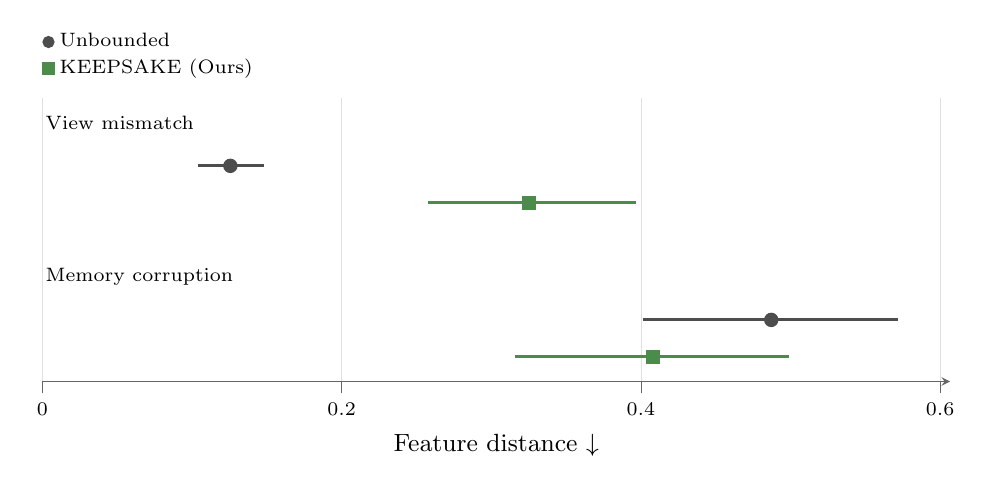
\begin{tikzpicture}
% Matched 60-s / 15-trajectory comparison; common baseline pixels.
\begin{axis}[
  scale only axis, width=\dimexpr\linewidth-17pt\relax, height=36mm,
  xmin=0.000000, xmax=0.606633, ymin=-0.28, ymax=1.56,
  ytick=\empty, xtick distance=0.2, scaled ticks=false,
  tick label style={font=\scriptsize}, label style={font=\small},
  xlabel={Feature distance $\downarrow$}, axis lines=left,
  y axis line style={draw=none}, axis line style={black!60}, tick style={black!60},
  tick align=outside, xmajorgrids=true, grid style={black!12,line width=0.25pt},
  clip=false, enlargelimits=false,
  legend style={font=\scriptsize,draw=none,fill=none,at={(0,1.05)},anchor=south west,
                legend columns=1,inner sep=0pt,row sep=-1pt},
  legend cell align=left,
]
\addlegendimage{only marks,mark=*,diagUnbounded}
\addlegendentry{Unbounded}
\addlegendimage{only marks,mark=square*,diagKeep}
\addlegendentry{KEEPSAKE (Ours)}
\node[anchor=west,font=\scriptsize,inner sep=1pt,fill=white]
  at (axis cs:0.000000,1.40) {View mismatch};
\node[anchor=west,font=\scriptsize,inner sep=1pt,fill=white]
  at (axis cs:0.000000,0.40) {Memory corruption};
\draw[diagUnbounded,line width=1.1pt] (axis cs:0.104065,1.12) -- (axis cs:0.147862,1.12);
\addplot[only marks,diagUnbounded,mark=*,mark size=2.4pt]
  coordinates {(0.125602,1.12)};
\draw[diagUnbounded,line width=1.1pt] (axis cs:0.401161,0.12) -- (axis cs:0.571633,0.12);
\addplot[only marks,diagUnbounded,mark=*,mark size=2.4pt]
  coordinates {(0.487087,0.12)};
\draw[diagKeep,line width=1.1pt] (axis cs:0.257853,0.88) -- (axis cs:0.396434,0.88);
\addplot[only marks,diagKeep,mark=square*,mark size=2.4pt]
  coordinates {(0.325372,0.88)};
\draw[diagKeep,line width=1.1pt] (axis cs:0.315901,-0.12) -- (axis cs:0.498888,-0.12);
\addplot[only marks,diagKeep,mark=square*,mark size=2.4pt]
  coordinates {(0.407863,-0.12)};
\end{axis}
\end{tikzpicture}
\endgroup

  \end{minipage}
  \caption{Retrieved-memory quality.}
  \label{fig:retrieval-quality-paired}
\end{subfigure}\hfill%
\begin{subfigure}[t]{0.32\linewidth}
  \centering
  \vspace{0pt}
  \begin{minipage}[c][60mm][c]{\linewidth}
    \centering
    % Generated by paper/export_memory_diagnostics_tikz.py.
% Requires \usepackage{pgfplots} and \pgfplotsset{compat=1.18}.
% Input inside a subfigure; do not resizebox the result (fonts would shrink).
\begingroup
\definecolor{diagKeep}{HTML}{4C8C4A}
\definecolor{diagFifo}{HTML}{D55E00}
\definecolor{diagUnbounded}{HTML}{4D4D4D}
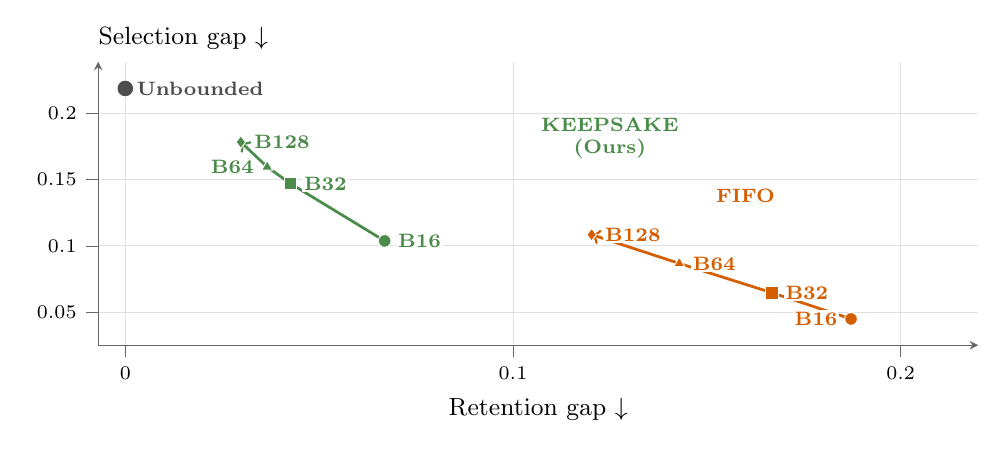
\begin{tikzpicture}
% Exact original 180-s / 13-trajectory rounded points, with RI omitted.
\begin{axis}[
  scale only axis, width=\dimexpr\linewidth-27pt\relax, height=36mm,
  xmin=-0.007, xmax=0.220, ymin=0.025, ymax=0.239,
  xtick={0,0.10,0.20}, ytick={0.05,0.10,0.15,0.20},
  scaled ticks=false,
  tick label style={font=\scriptsize,/pgf/number format/fixed,/pgf/number format/precision=2},
  label style={font=\small},
  xlabel={Retention gap $\downarrow$},
  axis lines=left, axis line style={black!60}, tick style={black!60},
  tick align=outside, grid=major, grid style={black!12,line width=0.25pt},
  clip=false, enlargelimits=false,
]
\node[anchor=south west,font=\small,inner sep=0pt]
  at (rel axis cs:0,1.04) {Selection gap $\downarrow$};
\addplot[diagFifo,line width=1pt,mark=none,->] coordinates {(0.1872,0.0448) (0.1668,0.0646) (0.1429,0.0867) (0.1203,0.1084)};
\addplot[only marks,diagFifo,mark=*,mark size=2.3pt,
  mark options={draw=white,line width=0.35pt,fill=diagFifo}] coordinates {(0.1872,0.0448)};
\node[anchor=east,font=\scriptsize\bfseries,text=diagFifo,
  inner sep=0.7pt,fill=white,xshift=-4pt]
  at (axis cs:0.1872,0.0448) {B16};
\addplot[only marks,diagFifo,mark=square*,mark size=2.3pt,
  mark options={draw=white,line width=0.35pt,fill=diagFifo}] coordinates {(0.1668,0.0646)};
\node[anchor=west,font=\scriptsize\bfseries,text=diagFifo,
  inner sep=0.7pt,fill=white,xshift=4pt]
  at (axis cs:0.1668,0.0646) {B32};
\addplot[only marks,diagFifo,mark=triangle*,mark size=2.3pt,
  mark options={draw=white,line width=0.35pt,fill=diagFifo}] coordinates {(0.1429,0.0867)};
\node[anchor=west,font=\scriptsize\bfseries,text=diagFifo,
  inner sep=0.7pt,fill=white,xshift=4pt]
  at (axis cs:0.1429,0.0867) {B64};
\addplot[only marks,diagFifo,mark=diamond*,mark size=2.3pt,
  mark options={draw=white,line width=0.35pt,fill=diagFifo}] coordinates {(0.1203,0.1084)};
\node[anchor=west,font=\scriptsize\bfseries,text=diagFifo,
  inner sep=0.7pt,fill=white,xshift=4pt]
  at (axis cs:0.1203,0.1084) {B128};
\addplot[diagKeep,line width=1pt,mark=none,->] coordinates {(0.0669,0.1037) (0.0426,0.1470) (0.0366,0.1596) (0.0298,0.1783)};
\addplot[only marks,diagKeep,mark=*,mark size=2.3pt,
  mark options={draw=white,line width=0.35pt,fill=diagKeep}] coordinates {(0.0669,0.1037)};
\node[anchor=west,font=\scriptsize\bfseries,text=diagKeep,
  inner sep=0.7pt,fill=white,xshift=4pt]
  at (axis cs:0.0669,0.1037) {B16};
\addplot[only marks,diagKeep,mark=square*,mark size=2.3pt,
  mark options={draw=white,line width=0.35pt,fill=diagKeep}] coordinates {(0.0426,0.1470)};
\node[anchor=west,font=\scriptsize\bfseries,text=diagKeep,
  inner sep=0.7pt,fill=white,xshift=4pt]
  at (axis cs:0.0426,0.1470) {B32};
\addplot[only marks,diagKeep,mark=triangle*,mark size=2.3pt,
  mark options={draw=white,line width=0.35pt,fill=diagKeep}] coordinates {(0.0366,0.1596)};
\node[anchor=east,font=\scriptsize\bfseries,text=diagKeep,
  inner sep=0.7pt,fill=white,xshift=-4pt]
  at (axis cs:0.0366,0.1596) {B64};
\addplot[only marks,diagKeep,mark=diamond*,mark size=2.3pt,
  mark options={draw=white,line width=0.35pt,fill=diagKeep}] coordinates {(0.0298,0.1783)};
\node[anchor=west,font=\scriptsize\bfseries,text=diagKeep,
  inner sep=0.7pt,fill=white,xshift=4pt]
  at (axis cs:0.0298,0.1783) {B128};
\addplot[only marks,diagUnbounded,mark=*,mark size=2.6pt]
  coordinates {(0,0.2188)};
\node[anchor=west,font=\scriptsize\bfseries,text=diagUnbounded,xshift=4pt,inner sep=0pt]
  at (axis cs:0,0.2188) {Unbounded};
\node[font=\scriptsize\bfseries,text=diagFifo,inner sep=1pt]
  at (axis cs:0.16,0.138) {FIFO};
\node[font=\scriptsize\bfseries,text=diagKeep,align=center,inner sep=1pt]
  at (axis cs:0.125,0.181) {KEEPSAKE\\(Ours)};
\end{axis}
\end{tikzpicture}
\endgroup

  \end{minipage}
  \caption{Retention--selection tradeoff.}
  \label{fig:retention-selection-tikz}
\end{subfigure}

% Suggested additions to the parent caption:
% (b) Matched 60-second reads (15 trajectories): mean clean-view mismatch
% and stored-content corruption (DINOv2 cosine distances), evaluated on
% common baseline pixels.
% Unbounded, FIFO B32, and KEEPSAKE B32 use the same matched queries.
% Whiskers are 95% trajectory-bootstrap intervals.
% (c) Original 180-second, 13-trajectory gap analysis, with budgets labeled.
% Lower is better on both axes; lines connect increasing budgets.
%
% For the temporal-change diagnostic, replace panel (b)'s input with
% tikz/retrieval_deterioration_comparison.tex and use this caption instead:
% Late-minus-early changes over sections 1--5 versus 19--23 of the matched
% 60-second suite; positive values indicate deterioration.
